\documentclass{article}

\usepackage[english]{babel}
\usepackage[a4paper,top=2cm,bottom=2cm,left=3cm,right=3cm,marginparwidth=1.75cm]{geometry}

\usepackage{amsmath}
\usepackage{graphicx}
\usepackage{minted}
\usepackage{parskip}

\usepackage[colorlinks=true, allcolors=blue]{hyperref}

\title{Solving 2048 with Expectimax}
\author{David Cook}

\begin{document}
\maketitle

\tableofcontents
\newpage
\begin{abstract}
The simplest goal of this project is to play the puzzle game 2048 with the expectimax algorithm. I intend to make it able to play any size of 2048 game, though eventually, any algorithm will break down if the grid is too large. In order to mitigate this, I intend to find ways of pruning the tree as much as possible. Officially the game of 2048 ends when the tile of 2048 finishes however the game can be continued until no more moves are possible.
\end{abstract}
\section{Introduction}
\label{sec:intro}
\subsection{The Problem}
\label{subsec:problem}
2048 is a game which features a 4x4 grid containing powers of 2. Each game starts with two cells, either 2 or 4.
All the tiles can be slid in any of the 4 directions at the same time. When two of the same powers of 2 collide the tiles merge, creating the next power of 2. The new tile increases the score by the value of the new tile. After each move, a new tile (either 2 or 4) will appear on the grid \cite{game2048}.

The goal of this project is to play a 2048 game using an AI-search algorithm. Previous projects have reached the tile of 8192 with reasonable consistency \cite{expectimax2048} but failed to go much higher. Reports were the rules of the game are changed are not very common, so the search algorithm shall play a $n \times m$ game rather than simply the traditional $4 \times 4$ 2048 game.

The most promising search algorithm is expectimax \cite{aiplays2048}. This is an algorithm designed for scenarios where there are two agents, one making random decisions and one making rational decisions \cite[~p.200]{russell2010artificial}. It is not practical to pre-compute a traditional 2048 decision tree, particularly when factoring in variable-size games.

\subsection{Deliverables}
\label{subsec:deliverable}
\subsubsection{Proof of concept programs}
\begin{enumerate}
    \item Decision Tree
    \item Simple Expectimax Example
    \item 2x2 2048 Game
    \item 2048 with a heuristic
\end{enumerate}
\subsubsection{Report}
\begin{enumerate}
    \item Design patterns in AI search.
    \item Techniques used by humans and previous automated solvers.
    \item User interface design for solver
    \item Complexity, NP-hardness and big $O$ notation
    \item The practicality and the effectiveness of the pruning expectimax tree.
    \item The heuristics have been generalised to support more 2048 games.
    \item Describe interesting algorithms and programming techniques, such as expectimax, used in the project.
    \item Implementation and performance of the decision tree.    
\end{enumerate}
The report will describe the implementation and optimisations of the expectimax algorithm, with a focus on any software engineering principles used in the processes. 
\subsubsection{Final Program}
\begin{enumerate}
    \item The final program will be written in java, with a full Object-oriented design, using modern software engineering principles.
    \item Theoretically capable of playing any $nxm$ 2048 game, though eventually break down due to performance.
    \item The program will have a user interface capable of keeping track of stats about the algorithms and an easy way of creating new $nxm$ games.
\end{enumerate}
\section{Proof of Concepts}
\label{sec:proof_of_concepts}
\subsection{Decision Tree}
\label{subsec:dt}
There are many ways of implementing a tree structure; various ones are more appropriate than others. The operations that a required in this situation are \cite{russell2010artificial}:
\begin{itemize}
    \item Generate a tree from the root node.
    \item Transverse the entire tree to calculate the score.
    \item Walk to a direct child node and regenerate the tree. At least the scores will need to regenerate on pre-existing nodes.
\end{itemize}
While this will likely not be true, I will assume generating a node can be done in $O(1)$ time. Generating or traversing nodes in a tree with $n$ nodes, can not be done in any less than $O(n)$. Reading a direct child can not be done in $O(1)$ time. \par
A common approach to making a tree is as follows:
\begin{minted}{java}
public class Node {
    int value;
    Node[] children;
}
\end{minted}
This is a node with an array of references to its child nodes. Traversing this entire tree will have a time complexity of 
$O(n)$. Arranging these nodes into a tree structure takes $O(n)$ and finally picking a direct child of a node takes $O(1)$,
Therefore there is no need to pick a less common tree implementation.

\subsection{Expectimax}
\label{subsec:expectimax}
\begin{figure}
    \centering
    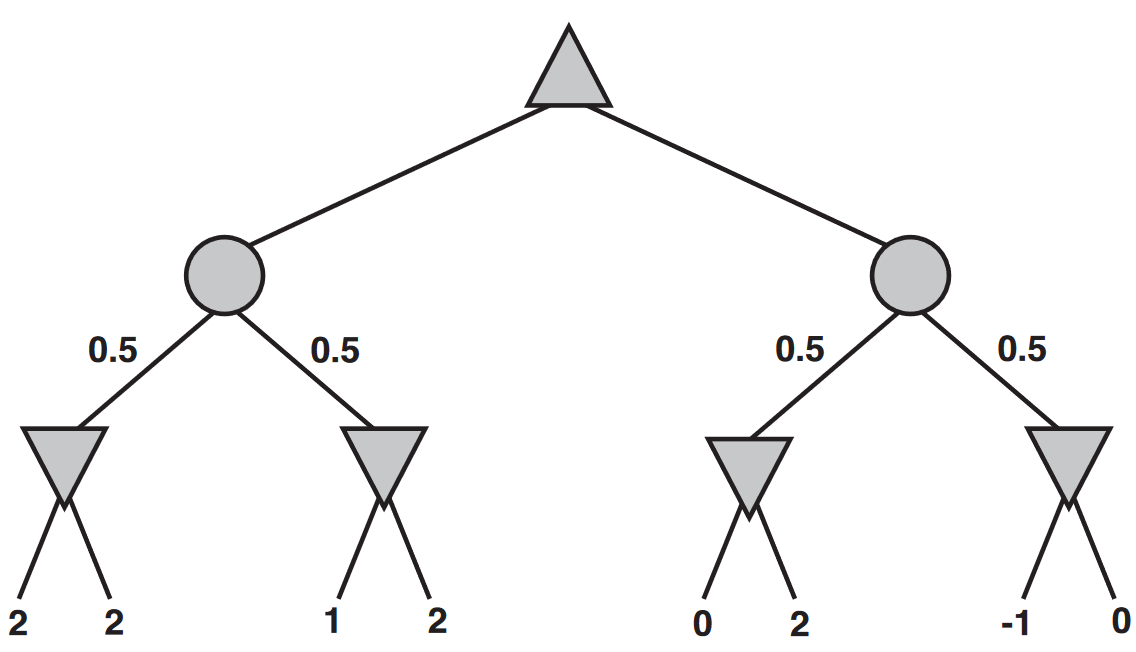
\includegraphics[width=0.7\textwidth]{expectimax.png}
    \caption{An image of an expectimax tree \cite[p.~200]{russell2010artificial}}
    \label{fig:expectree}
\end{figure}
The decision tree required in the expectimax algorithm (Figure \ref{fig:expectree}) has three types of nodes, however, only two types of nodes are needed for the problem of solving 2048. These three types of nodes include:
\begin{itemize}
    \item Maximizing nodes: These nodes get the maximum scoring child of the node, and acquire the same score
    \item Chance Nodes: These nodes represent situations where there are random states that may follow. The link weights between
    a chance node and its children represent the probability of that event occurring.
    \item Minimizing Nodes: These are the opposite of maximizing nodes, I do not expect to need them in this project.
    \item Terminus nodes: These nodes are the leaves of the tree. Their score is already known and used to calculate the score in the rest of the tree.
\end{itemize}
Each of these three relevant types of nodes has been converted to individual java classes, storing the scores in a float

attribute. This means that the value of the score only needs to be retrieved once.

\subsection{2048}
\label{subsec:2048}
This proof of concept was created mostly using one source \cite{source2048}, the original 2048 source code. While I did not
directly copy any of the code I read through most of the code relevant to the key features of the game and tried to understand 
why things were done that way. I then re-wrote the code in java using similar approaches.

I learnt a few things that were very useful while writing this prototype. For example: 
\begin{itemize}
    \item If you loop over the numbers in the wrong order a tile may collide with a tile that will be moved later. 
    See Figure \ref{fig:slidebug} for an example.
    \begin{figure}
        \centering
        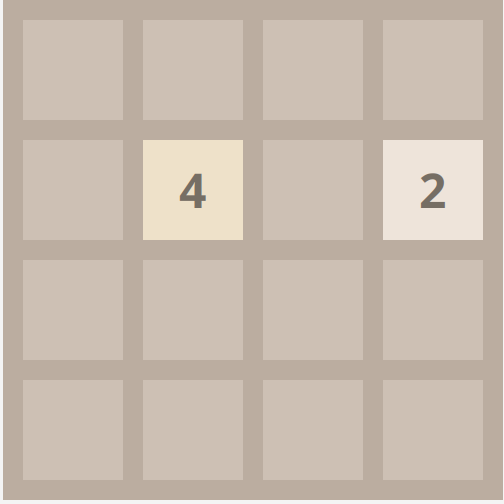
\includegraphics[width=0.3\textwidth]{2048_slide.png}
        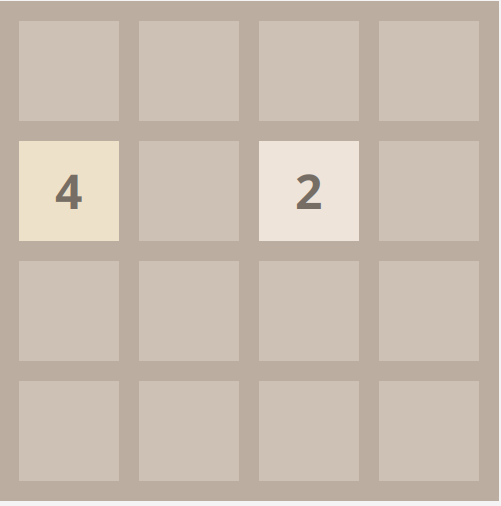
\includegraphics[width=0.3\textwidth]{2048_slide2.png}
        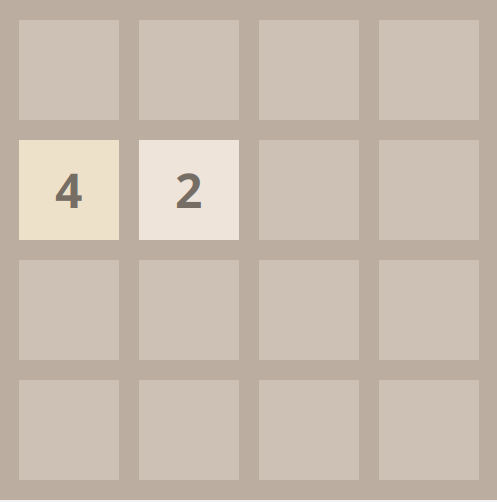
\includegraphics[width=0.3\textwidth]{2048_slide3.png}
        \caption{The first image shows a state where the bug can occur, second shows the bug, third shows what should happen}
        \label{fig:slidebug}
    \end{figure}
    \item When merging tiles you need to ensure that you do not merge a tile multiple times. See Figure \ref{fig:mergebug} for an example.
    \begin{figure}
        \centering
        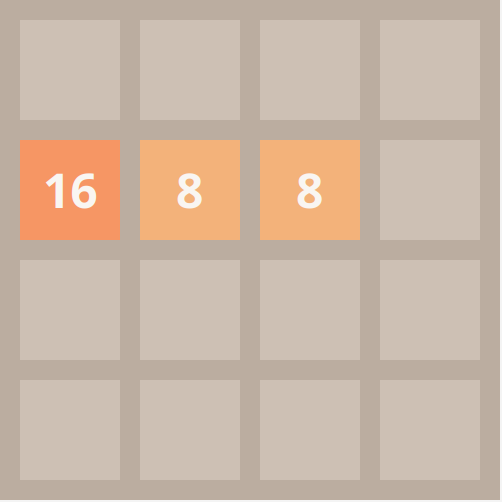
\includegraphics[width=0.3\textwidth]{2048_merge.png}
        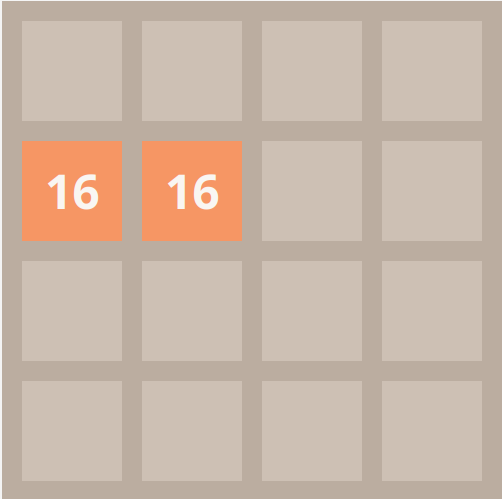
\includegraphics[width=0.3\textwidth]{2048_merge2.png}
        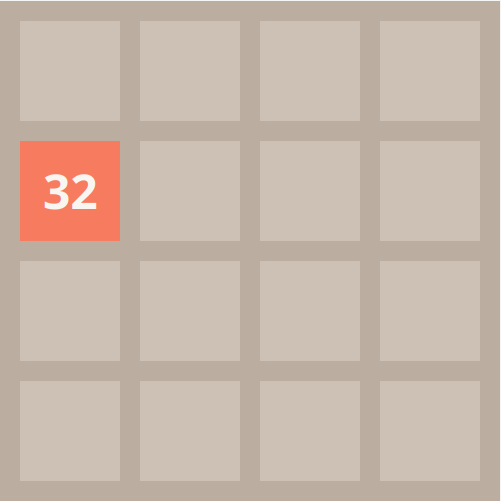
\includegraphics[width=0.3\textwidth]{2048_merge3.png}
        \caption{The first image shows a state where the bug can occur, second shows what should happen, third shows what happened after the bug occurs}
        \label{fig:mergebug}
    \end{figure}
\end{itemize}
The first bug was one that I was expecting to have to test for, however, I had not thought of the second case before writing the proof of concept. I only caught the second bug because I wrote a simple interface allowing me to play the game, and pick up on bugs.
\subsection{2048 with Expectimax}
\label{subsec:2048_expectimax}


\subsection{Heuristic for 2048}
\label{subsec:heuristic}


\section{User Interface Design}
\label{sec:ui}
\begin{figure}
    \centering
    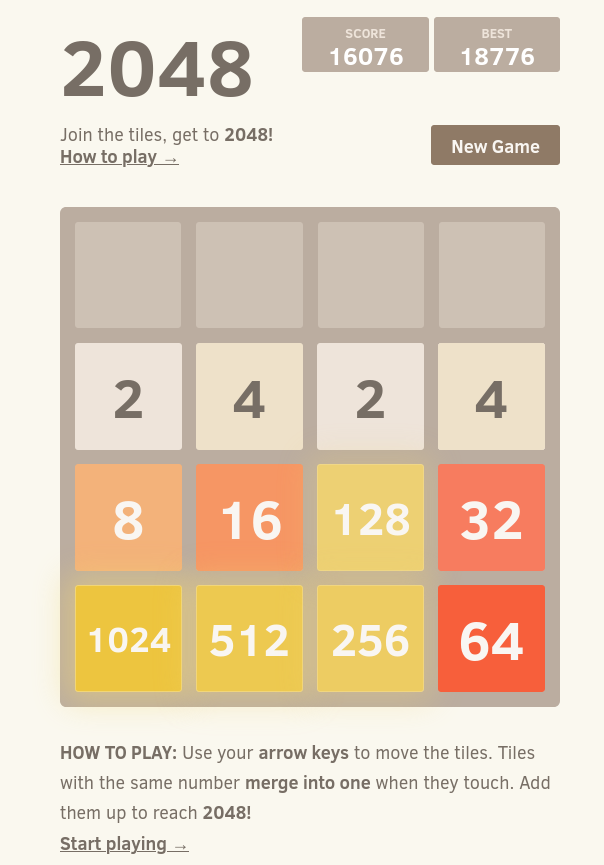
\includegraphics[width=0.4\textwidth]{2048-interface.png}
    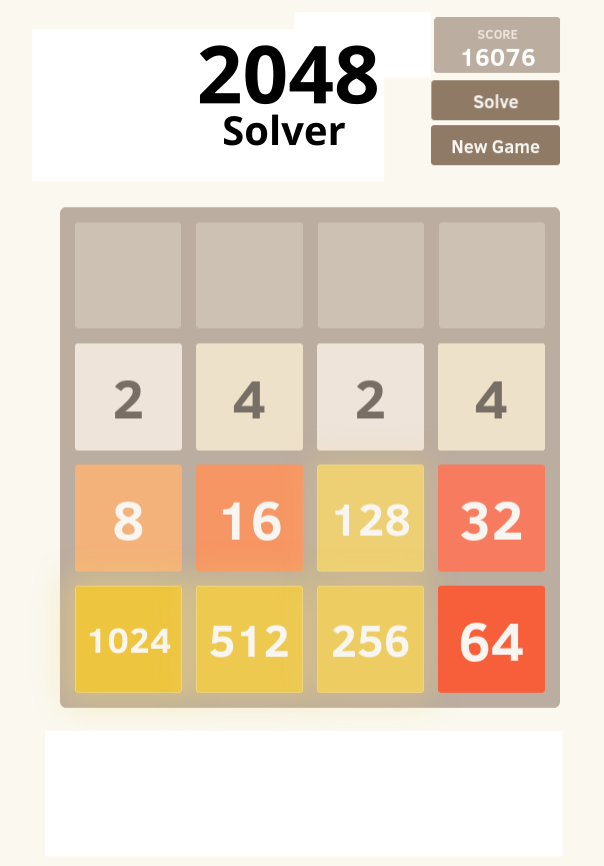
\includegraphics[width=0.4\textwidth]{interface-mockup.png}
    \caption{On the left is a screenshot of the official 2048 user interface \cite{game2048} and on the right
    is an edited version of this image designed to represent what my main interface might look like}
    \label{fig:2048interface}
\end{figure}
I would like the user interface to  resemble the original 2048 game, which can be seen in Figure. \ref{fig:2048interface}.
Parts of the user interface are appropriate for my solver. However, some features need to be removed, and other parts will need to be removed.

Firstly the instructions on how to play the game seen at both the top and bottom of the page can be removed
as the game will play itself. This means there will need to be a new solve button will need to be added.

I will also likely remove the 'best' score box from the interface. I will need to keep track of more data than the best score to evaluate how effective the algorithm is and will likely log this in a CSV file instead.

When the new game button is clicked, I will ask the user how big to make the game. This will be done with a dialogue asking the user how big the game is. When the gird is resized I will also change the minimum size of the window to ensure there is enough space for the game to be readable.

Most versions of 2048 have an animation that plays as the tiles slide; while this would be possible, as animations do exist in JavaFX \cite{javadocfx} however, I am not familiar with them, and think it is not worth the time to re-implementing the animations.

When creating a new game it is important that the user can enter the size of the new game however, this input should not be visible when the user doesn't want to make a new game. A long-established solution to this
is providing the user with a popup dialogue asking for the size of the game. There is no reference for this in the original 2048 to base the user interface on, so instead of modelling an existing interface, I have created a mock-up of what the interface should look like figure \ref{fig:popup}.

\begin{figure}
    \centering
    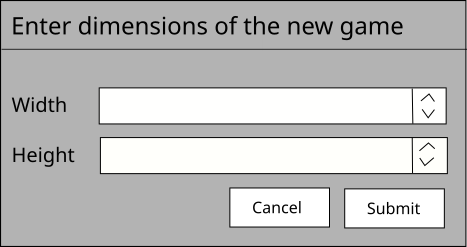
\includegraphics[width=0.4\textwidth]{newGamePopup.png}
    \caption{Mock up of the new game popup window.}
    \label{fig:popup}
\end{figure}
\section{Design Patterns for AI Search}
\label{sec:dp}

\section{Techniques used to solve the game}
\label{sec:techniques}

\subsection{Human Approaches}
\subsection{Automated Approaches}
\label{subsec:automated_techniques}

\section{Complexity}
\label{sec:complexity}

\subsection{Time Complexity}
\label{subsec:time_comp}

\subsection{NP Hardness}
\label{subsec:np_hardness}

\newpage
\bibliographystyle{IEEEtran}
\bibliography{refrences}
\end{document}